\documentclass[a4paper,oneside,article]{memoir}
\usepackage{fontspec}
  \setmainfont[Numbers=OldStyle,Ligatures=TeX]{Linux Libertine}
\usepackage[english,portuguese]{babel}
\usepackage{microtype,enumerate,graphicx,tikz,xtab,multirow,booktabs,array,pdfpages}
\usepackage[hidelinks]{hyperref}
\usetikzlibrary{mindmap,backgrounds}
\usepackage[alf,abnt-etal-list=4]{abntcite}

%% Faz referências etc.
\makeindex

%% Estilos: capítulo e página
\chapterstyle{article}
\makepagestyle{plain}
  \makeevenfoot{plain}{\thepage}{}{}
  \makeoddfoot{plain}{\thepage}{}{}
\pagestyle{plain}

%% Abreviações comuns
\newcommand{\unesp}{\textsc{unesp}}
\newcommand{\pibic}{\textsc{pibic}}
\newcommand{\celic}{\textsc{CELiC}}
\newcommand{\cnpq}{\textsc{cnp}q}
\newcommand{\icmc}{\textsc{icmc}}
\newcommand{\usp}{\textsc{usp}}
\newcommand{\nilc}{\textsc{nilc}}
\newcommand{\wnpr}{WN.Pr}
\newcommand{\wnbr}{WN.Br}
\newcommand{\eqsyn}{\textsc{eq\_syn\-o\-nym}}
\newcommand{\eqnsyn}{\textsc{eq\_near\_syn\-o\-nym}}
\newcommand{\eqhyper}{\textsc{eq\_has\_hyp\-ero\-nym}}
\newcommand{\eqhypo}{\textsc{eq\_has\_hyp\-o\-nym}}
\newcommand{\ili}{\textsc{ili}}
\newcommand{\en}[1]{\foreignlanguage{english}{#1}}

% Synset
\newcommand{\synset}[1]{\{~\textit{#1}~\}}

\begin{document}
\frenchspacing
%\OnehalfSpacing

%% Capa
  \begin{flushleft}
  {\large
  Programa \pibic/\cnpq/\unesp\\
  \textbf{Relatório Final}\\}
  (De 1\textordmasculine\ de março de~2011 a 31 de julho de 2012)\\
  \end{flushleft}

  \begin{flushright}
  Rafael Luis Beraldo\\
  {\small Bolsista}

  \vspace{1em}

  Bento Carlos Dias-da-Silva\\
  {\small Orientador}
  \end{flushright}

%% Citando
\nocite{cruse,bento,bentoetal,eurowordnet,fellbaum,ferreira,flexner,handke,houaissweb,houaiss,levin,marrafa,miller,saint,scott,taylor,vossen,weiszflog,wordnet,git,riemer,vossenetal}

%% Documento em si
\chapter{Introdução}

Este \textbf{Relatório Final} refere-se às atividades desenvolvidas pelo
bolsista Rafael Luis Beraldo no período de 1\textordmasculine~de março de~2011
a 31~de julho de~2012, após substituição da bolsista Débora Domiciano Garcia. O
Plano de Atividades em que este relatório se pauta sustenta-se no projeto do
orientador, \textit{``O Desenvolvimento da Base de Substantivos da WordNet.Br e
a sua Co-indexação com a WordNet de Princeton''}, que consiste na montagem de
parte da rede WordNet.Br (WN.Br) --- uma base relacional de unidades e
expressões lexicais do português do Brasil, construída a partir da investigação
de questões linguísticas~\cite{bentoetal,bento}, motivada pelo estudo da rede
WordNet de Princeton (WN.Pr), na versão \textit{WordNet 2.0}, e da metodologia
empregada em sua construção por pesquisadores do Laboratório de Ciências
Cognitivas da Universidade de Princeton, Estados
Unidos~\cite{miller,fellbaum}.\footnote{O termo \textit{wordnet} é
internacionalmente aceito para designar um tipo particular de base de
conhecimento lexical em que as relações que tecem a rede são relações
léxico-conceituais~\cite{marrafa}.} 

A WordNet.Br, como as demais wordnets, deverá constituir um recurso lexical
que, além de servir de instrumento complementar para o estudo de línguas,
poderá também ser utilizado em aplicações no âmbito do Processamento Automático
de Línguas Naturais (\textsc{pln}) e da Engenharia da Linguagem como, por
exemplo, sistemas de tradução automática, motores de busca na Internet (Google,
AltaVista, Lycos, entre outros), processadores e sumarizadores de texto,
aplicativos de recuperação de textos e de informação em bases de documentos e,
com a implementação do
\ili~(\foreignlanguage{english}{\textit{Inter-Lingual-Index}}), dicionários
digitais inglês--português/português--inglês para acesso gratuito online na
Internet.

Conforme os cronogramas de atividades (cf.~os~Planos do Bolsista em~Anexo), de
março de~2011 a~julho de~2012, coube ao bolsista a realização de tarefas que
permitiram o aprimoramento dos seus conhecimentos sobre o funcionamento das
redes wordnet norte-americana e europeias, e a sua contribuição para o
desenvolvimento da rede wordnet brasileira.

As atividades de pesquisa deste projeto realizaram-se no \celic\ (Centro de
Estudos Linguísticos e Computacionais da Linguagem), localizado na Sala~29,
Prédio dos GPs, Faculdade de Ciências e Letras, \unesp, Campus de Araraquara,
sede do Grupo de Pesquisa ``Grupo de Estudos Linguístico-Computacionais da
Linguagem Humana'', liderado pelo orientador, cadastrado no \cnpq\ e
certificado pela Universidade.

\chapter{Objetivos}

Os principais objetivos das atividades do bolsista, previstos no Plano de
Atividades para o período de~março de~2011 a~julho de~2012, incluíram:

\begin{enumerate}[a.] \item Estudar os tópicos de semântica lexical referentes
      à classe dos substantivos, selecionados da Bibliografia Básica;

  \item\label{item} Proceder à análise léxico-semântica dos synsets do
    português extraídos da base da WordNet.Br. (em construção), a partir da
    projeção da análise de mesma natureza de 700~synsets (números~300--499 e
    números~1000--1499) de substantivos do arquivo de base
    \texttt{06artifact(11256).doc} do inglês, extraídos da base da WordNet de
    Princeton, dando continuidade ao trabalho de análise anterior;

  \item Para cada synset do português selecionado em~(\ref{item}), analisar a
    sua boa-formação gráfica e a sua consistência léxico-conceitual, ou seja,
    corrigir os itens lexicais mal-grafados e verificar se todos eles
    lexicalizam um mesmo conceito; atividade de análise que se realiza pautada
    nos estudos de semântica lexical, na análise das concordâncias e na
    consulta aos dicionários Webster's eletrônico, \textsc{rhud}, Michaelis,
    Aurélio e Houaiss referidos na Bibliografia Básica; caso seja necessário,
    novos synsets do português são criados nesse processo;

  \item Participar de encontros semanais de orientação;

  \item Elaborar relatório científico e produzir um trabalho para a
    apresentação em congresso de \textsc{ic}.
\end{enumerate}

\chapter{Metodologia}

Nessa seção listaremos os fundamentos teórico-aplicados utilizados na análise
dos synsets, bem como elucidaremos as estratégias e convenções dessa análise.
Esses dois aspectos da metodologia do projeto permitem o estabelecimento de um
estilo padrão para os synsets da \wnbr. Também discutiremos, na sequência, a
implementação do Git~\cite{git}, software que foi selecionado para otimizar o
armazenamento e o gerenciamento dos diferentes tipos de arquivo que são gerados
na execução das atividades de construção da \wnbr.

\section{Metodologia de base}

Antes que qualquer análise de synsets seja feita, é necessário compreender os
aspectos teóricos por trás da \wnpr, produzida para o inglês norte-americano,
os pressupostos para o alinhamento de wordnets e as particularidades da \wnbr.
Essa necessidade foi suprida com o estudo dos textos da Bibliografia Básica.

Destacamos alguns textos fundamentais, como~\citeonline{fellbaum}, que descreve
minuciosamente a WN.Pr, e~\citeonline{vossen}, uma edição especial do periódico
\en{\textit{Computers and the Humanities}}, que discute as dificuldades e
estratégias na construção da EuroWordNet, uma mega-WordNet multilíngue, que
associa diferentes wordnets em construção para as línguas da União Europeia.
Incluímos nessa lista~\citeonline{riemer}, que fornece o embasamento teórico
que precedeu àquele dos textos acima, discutindo teorias e conceitos da
semântica (geral e lexical) que se provaram bastante úteis na compreensão das
wordnets, em especial o capítulo~8.

\section{Estratégias de execução}

De acordo com os fundamentos teóricos fornecidos pela Bibliografia Básica, para
cada synset selecionado da base da WN.Br, após análise léxico-semântica,
propõe-se uma glosa.

A metodologia adotada apresentou grande eficiência, o que tornou desnecessária a
modificação dos procedimentos ao longo dos trabalhos.

Procedimentos:
	
\begin{enumerate}
  \item Iniciam-se os seguintes aplicativos:

    \begin{enumerate}[a.]
      \item \texttt{06artifact(11256).doc};
      \item Arquivo modelo para posterior indexação (\texttt{.txt});
      \item WordNet 2.0;
      \item Editor da \wnbr;
      \item Dicionários de inglês/inglês e inglês/português;
      \item Navegador de internet com acesso ao córpus (\nilc) e à
        ferramentas de busca (Google, AltaVista, Yahoo).
    \end{enumerate}

  \item\label{selecao_synset} Seleciona-se o synset do inglês que dará origem à
    análise ou construção do synset do português na lista de synsets do
    tipo~\texttt{06artifact(11256).doc} e localiza-se esse synset na base da
    WN.Pr; todo seu conteúdo (o synset e todas as informações associadas a ele,
    incluindo todos os seus hiperônimos) é copiado para o arquivo modelo em
    \texttt{.txt}. Cada synset da~\wnpr\ constitui um \ili\
    (\en{Inter-Ligual-Index}), ou seja, um indexador que se alinha (associa) a
    um ou mais synsets conceitualmente equivalentes do português e funciona
    como elo de ligação (indexado, portanto) a synsets conceitualmente
    equivalentes de outras línguas.

  \item\label{analise_synset} Copia-se o synset do português semanticamente
    equivalente ao inglês, se ele já existir na base da WN.Br, para o arquivo
    referido em~\ref{selecao_synset}, analisando-o quanto à sua boa-formação
    ortográfica e semântico-conceitual (esta análise consiste em:  ampliar ou
    reduzir o synset, segmentá-lo em dois ou mais synsets ou excluí-lo da base
    do português); caso não haja um synset equivalente na base do português,
    constrói-se um novo synset que se alinhe conceitualmente ao synset do
    inglês referido em~\ref{selecao_synset}, ou seja, procura-se construir o
    synset português cujas unidades lexicais sejam traduções das unidades
    lexicais do synset do inglês.

  \item Durante os procedimentos em~\ref{analise_synset}, observa-se qual
    destas análises que, previstas em~\citeonline{vossenetal}, será a mais
    apropriada para especificar o alinhamento conceitual que resulta da
    análise: alinhamento por \eqsyn, por \eqnsyn, por \eqhypo\ ou por \eqhyper.

  \item Cria-se a glosa para o synset do português em construção, com base na
    glosa já existente para o synset do inglês, quando esta já estiver
    especificada no synset do inglês.

  \item Para cada unidade lexical que constitui o synset do português,
    selecionam-se frases-exemplo em corpus. As frases localizada no corpus do
    Núcleo Interinstitucional de Linguística Computacional~\cite{nilc} têm
    prioridade sobre as frases localizadas pelas ferramentas de busca da web;
    usa-se o critério de maior frequência de ocorrência da unidade lexical em
    corpora para decidir a seleção das frases-exemplo; quando a frase é selecionada
  na web, sinaliza-se o fato, acrescentando-se ``\texttt{I]}'' (``proveniente da
  Internet'') a unidade lexical da frase que corresponde à unidade lexical do
  synset.

\item Define-se a chave do synset, que é a unidade lexical pertencente a ele e
  que é a mais frequente na busca em corpus ou a intuitivamente mais usada.

\item Conclui-se a análise e nomeia-se o arquivo segundo este padrão:

  \begin{center}
    \texttt{<n\textordmasculine\_na\_Base\_WNBr>.<ILI>.<tipo\_semântico>.
    <chave>.void|md|cr.HYPER|HYPO|NEAR|void>}
  \end{center}

\end{enumerate}

\section{Estratégia de gerenciamento dos arquivos}

A dimensão do desafio que é gerenciar a base de arquivos da~\wnbr\ pode ser
apreciada considerando-se que, entre~2010 e~2012, foram produzidos e revistos
certa de~4100 arquivos, correspondendo ao mesmo número de synsets produzidos e
alinhados. Cinco bolsistas de~\textsc{ic}, supervisionados pelo coordenador,
estiveram envolvidos nas tarefas, que significaram a exploração de diferentes
análises até a escolha final de cada synset considerado ideal para configurar
na base da~\wnbr; análises cujos históricos foram documentados para que toda e
qualquer decisão analítica pudesse ser recuperada, revista e atualizada.

A solução em teste para o desafio é a adoção do~Git, um sistema de controle de
versões de arquivos~\cite{chacon}, que deve viabilizar:

\begin{enumerate}
  \item O controle do histórico da construção e do alinhamento de synsets (Que
    análise foi feita? Quem a fez? Quando?);
  \item O registro de análises distintas para o mesmo synset, resultando em
    alinhamentos diferentes;
  \item O acesso, via Internet, a todos os arquivos gerados pelos
    desenvolvedores do projeto, pois cada desenvolvedor pode copiar todos os
    arquivos da base da \wnbr\ (no servidor) para a sua máquina local durante o
    seu trabalho, utilizar aqueles que são relevantes para as suas análises sem
    interferir na integridade dos mesmos, pois trabalha com uma cópia e seu
    acesso é restrito no servidor;
  \item A marcação e o resgate de uma versão do arquivo que registra o synset e
    o seu alinhamento considerados ideais;
  \item A consolidação da base da~\wnbr.
\end{enumerate}

Cumpre destacar que um Sistema de Controle de Versões~(SCV) resolve todos esses
problemas, permitindo ao usuário reverter seus arquivos a um estado anterior,
reverter todo seu trabalho a um estado anterior, comparar as mudanças ao longo
do tempo, ver quem foi o último a modificar os arquivos, e recuperar arquivos
que foram comprometidos ou apagados por acidente\footnote{\citeonline{chacon}:
\url{http://git-scm.com/book/en/Getting-Started-About-Version-Control}}.

A escolha do sistema de controle de versões~Git foi motivada por ser rápido,
estável, possuir todas as características apontadas acima e por sua licença de
software livre\footnote{\url{https://github.com/git/git/blob/master/COPYING}}.
Prova de que o~Git é capaz de gerenciar a base da~\wnbr\ é sua história. O
programa foi criado, originalmente, para gerenciar as mudanças no~Linux,
projeto para o qual mais de~7800 pessoas e quase~800 empresas já
contribuíram~\cite[p.~1]{corbetetal}.

Durante reuniões no final de~2010 e início de~2011, foram discutidos os
detalhes iniciais para a implementação do Git~\cite[p.~4]{beraldo11}. O Git foi
implementado e testado, usando um servidor cedido pelo~\nilc, no~\icmc\
(Instituto de Ciências Matemáticas e Computação) da \usp\ de São Carlos. Em
reunião no final de julho, foi decidido o deslocamento do repositório da~\wnbr\
do atual servidor, que é de acesso privado no~\nilc, para o servidor de acesso
público no~GitHub\footnote{\url{https://github.com/}}. Essa iniciativa busca
promover a divulgação do projeto e, sobretudo, dos resultados, à medida que
forem sendo consolidados, bem como promover a comunicação entre os
pesquisadores e demais interessados na construção e uso da~\wnbr. A
figura~\ref{github:repositorio} mostra a interface de um repositório
configurado no~GitHub.

%% Imagem da interface geral de um repositório no GitHub
\begin{figure}[h]
  \centering
  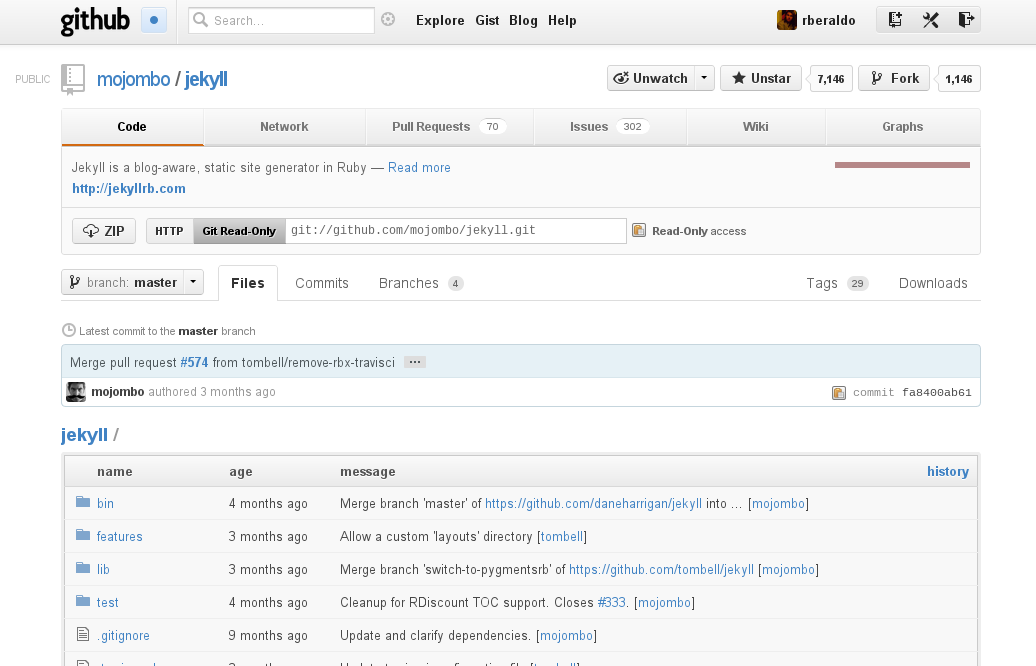
\includegraphics[width=.9\textwidth]{img/repositorio.png}
  \caption{A interface de um repositório no GitHub}
  \label{github:repositorio}
\end{figure}

No GitHub é possível adicionar pessoas a um projeto, para que possam
contribuir ativamente; o único pré-requisito é que possuam uma conta no GitHub.
Também é possível aceitar alterações e melhorias em geral (\en{\textit{“pull
requests”}}) de outros usuários do GitHub. Desse modo, tem-se o controle de
quem fez uma modificação ou adição, ou mesmo apagamento de informações e
arquivos, quando foi feita e por qual motivo. O sistema do GitHub também
permite que usuários copiem para suas contas o estado atual do projeto sem que
nenhuma modificação seja feita nos arquivos originais. Usuários não cadastrados
também podem fazer uma cópia local dos arquivos. Em nenhum desses casos há a
possibilidade de alteração da base por pessoas não autorizadas.

Além disso, o GitHub possui um serviço de Wiki~(figura~\ref{github:wiki}) e um
sistema de comunicação de \en{\textit{bugs}}, ou seja, erros ou problemas
(figura~\ref{github:bugtracker}).

 %% Imagem da wiki do Github
 \begin{figure}[h]
   \centering
   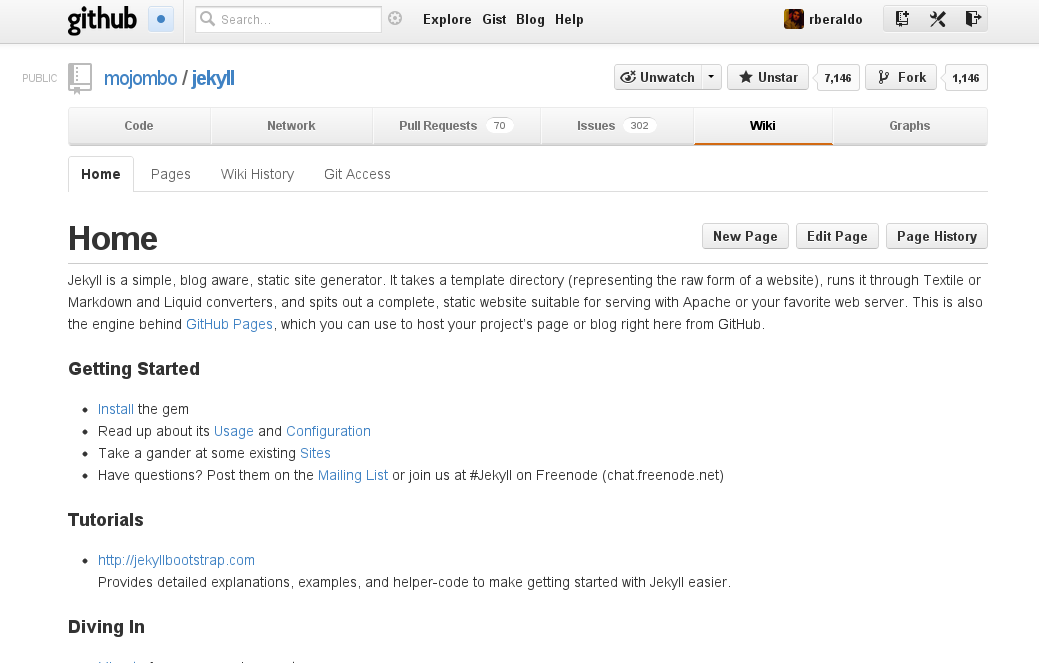
\includegraphics[width=.9\textwidth]{img/wiki.png}
   \caption{A Wiki fornecida pelo GitHub pode conter a documentação do projeto}
   \label{github:wiki}
 \end{figure}
 
 %% Imagem do bugtracker do GitHub
 \begin{figure}[h]
   \centering
   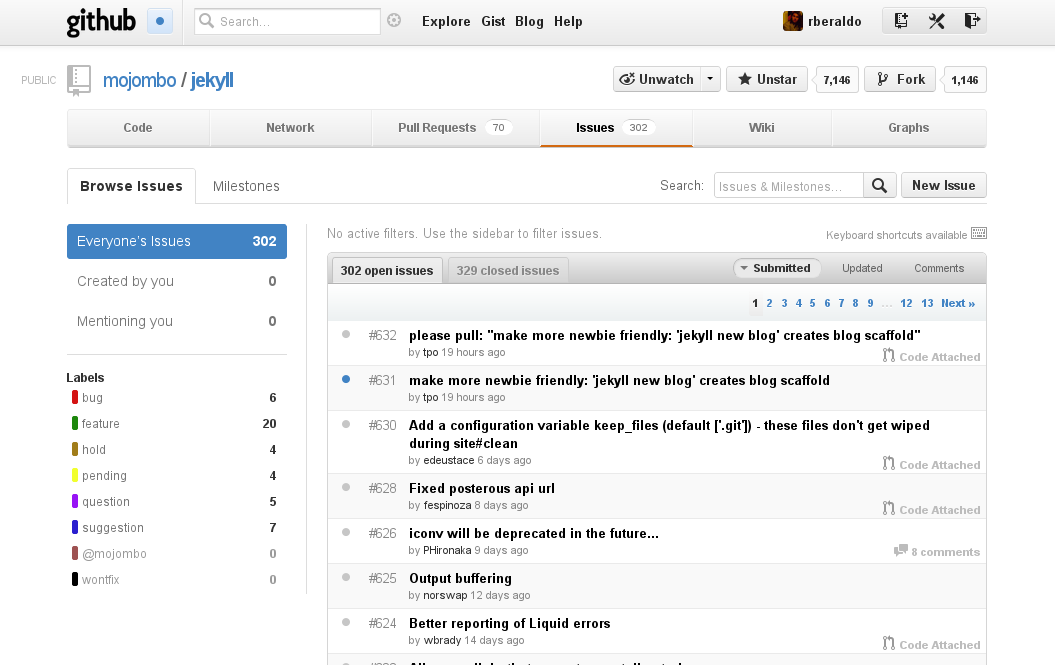
\includegraphics[width=.9\textwidth]{img/bugtracker.png}
   \caption{O \en{\textit{bug tracker}} fornecido pelo GitHub pode ajudar a resolver problemas na \wnbr}
   \label{github:bugtracker}
 \end{figure}

A área de ajuda do GitHub\footnote{\url{https://help.github.com/}} possui uma
página explicando a configuração necessária para acessar os repositórios
disponíveis em todo o
site\footnote{\url{https://help.github.com/articles/set-up-git}}, que difere em
cada sistema operacional. A área também possui uma parte dedicada ao uso do
Git\footnote{\url{https://help.github.com/categories/19/articles}}, onde o
usuário pode encontrar referências, entre livros e vídeos, que explicam o fluxo
do trabalho usando os vários clientes disponíveis para o Git, dos mais
tradicionais, como a linha de comando, aos mais amigáveis para o usuário, como
os clientes fornecidos pelo GitHub\footnote{Cliente para Windows disponível em
\url{http://windows.github.com/} e para Mac em \url{http://mac.github.com/}}.

Com a adoção do sistema de controle de versões Git e do servidor de acesso
público do GitHub, espera-se maior agilização da construção, do armazenamento,
da revisão e da atualização da base da~\wnbr\ e, sobretudo, a sua
disponibilização para os usuários e as suas periódicas atualizações.

\chapter{Resultados}

% Original adaptado do Filipe
% Ao fim de um ano e cinco meses de trabalho, verifica-se o cumprimento de todos
% os objetivos programados para esse período, incluindo o aprofundamento dos
% conhecimento teóricos e metodológicos, concentrados em textos selecionados
% de~\cite{cruse}, \cite{fellbaum}, \cite{marrafa}, \cite{vossen},
% \cite{vossenetal} e~\cite{bento}; a realização do trabalho aplicado de
% alinhamento entre substantivos das duas bases, proporcionando ao bolsista a
% oportunidade de adquirir experiências em desenvolver pesquisa teórico-empírica,
% e também o conhecimento relacionado às wordnets norte-americana e europeia ---
% a EuroWordNet, uma rede semântica que inter-relaciona as wordnets das línguas
% da União Européia.

% Minha versão para comportar as tabelas
Ao fim de um ano e cinco meses de trabalho, verifica-se o cumprimento de todos
os objetivos programados para esse período, incluindo o aprofundamento dos
conhecimento teóricos e metodológicos, a realização do trabalho aplicado de
alinhamento entre substantivos das duas bases~(WN.Br e WN.Pr), o que
proporcionou ao bolsista a oportunidade de adquirir experiências em desenvolver
pesquisa teórico-empírica, e também os conhecimentos necessários para o
desenvolvimento de wordnets.

O quadro~\ref{panorama0} resume os objetivos para os primeiros cinco~meses de
trabalho; o quadro~\ref{panorama1} apresenta os objetivos para os doze meses
finais. Os quadros foram retirados dos Anexos~1 e~2, respectivamente. Os
Apêndices~1 e~2 apresentam, sob a forma de tabelas, os resultados obtidos
durante o período da bolsa: todos os synsets e glosas construídos para o
português, com os seus respectivos alinhamentos aos synsets do inglês.

% Tabela dos primeiros cinco meses
\begin{table}[!h]\footnotesize
  \centering
  \begin{tabularx}{\linewidth}{ l X X } 
    \toprule
    \textbf{Ao final de} & \textbf{Realizar as atividades} & \textbf{Com a previsão dos seguintes resultados} \\
    \midrule
    5 meses & Além dos estudos teórico-metodológicos, as atividades incluem,
sobretudo, a especificação das frases-exemplos para cada um dos itens lexicais
constitutivos de cada synset do português que puder ser indexado a cada um dos
200 synsets do inglês~(\textsc{artifact}), a análise, a revisão e a glosagem
dos synsets de substantivos do português e o seu alinhamento ao respectivo
synset do inglês (a indexação). & Domínio das técnicas de análise
léxico-semântica, inserção dos synsets indexados na base da WordNet.Br,
estabelecendo da correspondência entre estes e os seus equivalentes semânticos
na WordNet de Princeton e a especificação das relação de antonímia, hiponímia e
meronímia entre os synsets do português, contribuindo assim para a construção
da base dos substantivos do domínio~\textsc{artifact} da WordNet.Br.~(00300 a
00499) \\
    \bottomrule
  \end{tabularx}
  \caption{Panorama dos primeiros cinco meses}
  \label{panorama0}
\end{table}

% Tabela dos últimos doze meses
\begin{table}[!h]\footnotesize
  \centering
  \begin{tabularx}{\linewidth}{ l X X } 
    \toprule
    \textbf{Ao final de} & \textbf{Realizar as atividades} & \textbf{Com a previsão dos seguintes resultados} \\
    \midrule
    12 meses & Além dos estudos teórico-metodológicos, as atividades incluem,
sobretudo, a especificação das frases-exemplos para cada um dos itens lexicais
constitutivos de cada synset do português que puder ser indexado a cada um dos
200 synsets do inglês~(\textsc{artifact}), a análise, a revisão e a glosagem
dos synsets de substantivos do português e o seu alinhamento ao respectivo
synset do inglês (a indexação). & Domínio das técnicas de análise
léxico-semântica, inserção dos synsets indexados na base da WordNet.Br,
estabelecendo da correspondência entre estes e os seus equivalentes semânticos
na WordNet de Princeton e a especificação das relação de antonímia, hiponímia e
meronímia entre os synsets do português, contribuindo assim para a construção
da base dos substantivos do domínio~\textsc{artifact} da WordNet.Br.~(01000 a
01499) \\
    \bottomrule
  \end{tabularx}
  \caption{Panorama dos doze meses finais}
  \label{panorama1}
\end{table}

%\begin{table}[h]\footnotesize
%\tablefirsthead{\toprule \textbf{\ili/número na base} & \textbf{Relação semântica} & \textbf{WordNet.Br} & \textbf{WordNet.Pr} \\ \midrule}
%\tablehead{\toprule \textbf{\ili/número na base} & \textbf{Relação semântica} & \textbf{WordNet.Br} & \textbf{WordNet.Pr} \\}
%\tabletail{\bottomrule}
%  \begin{xtabular}[h]{m{.15\textwidth} m{.25\textwidth} m{.22\textwidth} m{.22\textwidth}}
%    02626354 & \eqsyn & \synset{antifúngico, agente antifúngico, fungicida, antimicótico, agente antimicótico} & \synset{\en{antifungal, antifungal agent, fungicide, antimycotic, antimycotic agent}} \\
%    \hline
%    02626693 & \eqsyn & \synset{traje anti-G} & \synset{\en{anti-G suit, G suit}} \\
%    \hline
%    02626842 & \eqsyn & \synset{anti-histamínico} & \synset{\en{antihistamine}} \\
%    \hline
%    02627277 & \eqsyn & \synset{antihipertensivo, droga antihipertensiva} & \synset{\en{antihypertensive, antihypertensive drug}} \\
%    \hline
%    02627637 & \eqsyn & \synset{anti-inflamatório, droga anti-inflamatória} & \synset{\en{anti-inflammatory, anti-inflammatory drug}} \\
%    \hline
%    02627912 & \eqhypo & \synset{capa protetora} & \synset{\en{antimacassar}} \\
%    \hline
%    02628045 & \eqsyn & \synset{antimalárico, droga antimalárica} & \synset{\en{antimalarial, antimalarial drug}} \\
%    \hline
%    02628263 & \eqsyn & \synset{antimetabólito} & \synset{\en{antimetabolite}} \\
%    \hline
%    02628446 & \eqsyn & \synset{antimicina} & \synset{\en{antimycin}} \\
%    \hline
%    02628555 & \eqsyn & \synset{antineoplásico, droga antineoplásica, medicamento anticancerígeno} & \synset{\en{antineoplasic, antineoplasic drug, cancer drug}} \\
%    \hline
%    02629076 & \eqsyn & \synset{antibiótico antineoplásico} & \synset{\en{antineoplasic antibiotic}} \\
%    \bottomrule
%  \end{xtabular}
%  \caption{Síntese dos primeiros cinco meses}
%  \label{synsets0}
%\end{table}
%
%%%%%%%%%%%%%%% SEGUNDA PARTE %%%%%%%%%%%%%%%
%
%\begin{table}[h]\footnotesize
%\tablefirsthead{\toprule \textbf{\ili/número na base} & \textbf{Relação semântica} & \textbf{WordNet.Br} & \textbf{WordNet.Pr} \\ \midrule}
%\tablehead{\toprule \textbf{\ili/número na base} & \textbf{Relação semântica} & \textbf{WordNet.Br} & \textbf{WordNet.Pr} \\}
%\tabletail{\bottomrule}
%  \begin{xtabular}[h]{m{.15\textwidth} m{.25\textwidth} m{.22\textwidth} m{.22\textwidth}}
%    02741864 & \eqsyn & \synset{laboratório de biologia} & \synset{\en{biology lab, biology laboratory, bio lab}} \\
%    \hline
%    02741989 & \eqsyn & \synset{bioscópio} & \synset{\en{bioscope}} \\
%    \hline
%    02742159 & \eqsyn & \synset{arma biológica} & \synset{\en{bioweapon, biological weapon, bioarm}} \\
%    \hline
%    02742429 & \eqsyn & \synset{biplano} & \synset{\en{biplane}} \\
%    \hline
%    02742540 & \eqsyn & \synset{biprisma} & \synset{\en{biprism}} \\
%    \hline
%    02742801 & \eqsyn & \synset{canoa de casca de bétula} & \synset{\en{birchbark canoe, birchbark, birch bark}} \\
%    \hline
%    02742930 & \eqsyn & \synset{banho de pássaro, banho de ave} & \synset{\en{birdbath}} \\
%    \hline
%    02743048 & \eqsyn & \synset{gaiola} & \synset{\en{birdcage}} \\
%    \hline
%    02743321 & \eqsyn & \synset{casa de passarinho} & \synset{\en{birdhouse}} \\
%    \hline
%    02743414 & \eqsyn & \synset{munição para caça} & \synset{\en{bird shot, buckshot, duck shot}} \\
%    \hline
%    02743546 & \eqsyn & \synset{barrete} & \synset{\en{biretta}} \\
%    \hline
%    02743671 & \eqsyn & \synset{bispo} & \synset{\en{bishop}} \\
%    \hline
%    02743829 & \eqsyn & \synset{bistrô} & \synset{\en{bistro}} \\
%    \hline
%    02743922 & \eqsyn & \synset{broca} & \synset{\en{bit}} \\
%    \hline
%    02744329 & \eqsyn & \synset{freio} & \synset{\en{bit}} \\
%    \hline
%    02744617 & \eqsyn & \synset{placa de mordida} & \synset{\en{bite plate, biteplate}} \\
%    \hline
%    02745628 & \eqsyn & \synset{preto} & \synset{\en{black}} \\
%    \hline
%    02745747 & \eqsyn & \synset{preta} & \synset{\en{black }} \\
%    \hline
%    06267282 & \eqsyn & \synset{preto-e-branco} & \synset{\en{print, black and white}} \\
%    \hline
%    02745998 & \eqsyn & \synset{lousa, quadro, quadro-negro} & \synset{\en{blackboard, chalkboard}} \\
%    \bottomrule
%  \end{xtabular}
%  \caption{Síntese dos doze meses finais}
%  \label{synsets1}
%\end{table}

\pagebreak
\chapter{Discussão}

% Introdução à terminologia
Na busca de um synset do português que seja conceitualmente equivalente ao do
inglês, nem sempre ocorre um alinhamento direto, devido às especificidades de
cada uma das línguas e, sobretudo, às lacunas lexicais que são constatadas
durante o processo de análise.

%\enlargethispage{\baselineskip}
Segundo~\citeonline{peters}, há seis tipos de relações interlinguais. O
alinhamento direto é chamado~\eqsyn. As outras relações mais importantes
são~\cite[p.~225, tradução livre]{peters}:

	\begin{itemize}
        \item \eqnsyn\ quando um sentido corresponde a vários \ili s
          simultaneamente;
        \item \eqhyper\ quando um sentido é mais específico que qualquer \ili\
          disponível;
        \item \eqhypo\ quando um sentido pode ser ligado apenas a \ili s mais
          específicos.
	\end{itemize}

% Exemplos de alinhamento direto
Exemplo de \eqsyn\ é o synset da \wnpr\ \synset{\en{bread knife}}, que se
alinha diretamente com o synset da \wnbr\ \synset{faca de pão}. Nesse caso,
verificamos que as duas línguas --- o inglês norte-americano e o português
brasileiro --- revestem lexicalmente o mesmo conceito \textsc{faca especial
  para cortar pães}.

Mesmo que esse tipo de alinhamento pareça bastante simples, existem algumas
questões a serem levantadas. Algumas são de cunho linguístico e se relacionam
às especificidades de cada língua, como no caso do synset \synset{\en{brush2}}
da \wnpr. Nesse caso, o synset reveste lexicalmente o conceito
\textsc{utensílio que tem pelos ou cerdas firmemente presas a um cabo}. No
português brasileiro, existem ao menos dois possíveis synsets que revestem esse
conceito: \synset{escova} e \synset{pincel}. A dificuldade deriva do fato que,
em português, o conceito é bipartido em função do uso das escovas e pincéis;
podemos pensar que escovas \emph{limpam} ao passo que pincéis \emph{espalham}
(tinta, claras de ovos etc.). No inglês, essa diferenciação conceitual é
lexicalizada por synsets contendo itens léxicos complexos: \synset{\en{cleaning
brush}} e \synset{\en{paint brush}}.

Outro tipo de problema decorre de possíveis problemas na formação dos synsets
da \wnpr. Esse é o caso de \synset{\en{bitmap, electronic image}}. Aqui é
necessária a compreensão técnica do termo “\en{\textit{bitmap}}”.
Segundo~\cite{wiki_bitmap}:

\begin{quote}
  [\ldots]~\en{bitmap or pixmap is a type of memory organization or image file
    format used to store digital images. The term bitmap comes from the computer
    programming terminology, meaning just a map of bits, a spatially mapped array
  of bits.}
\end{quote}

A dificuldade está, portanto, na concepção de \textit{\en{bitmap}} enquanto um
tipo de imagem digital. Acreditamos que, por esse motivo, o synset
\synset{\en{bitmap}} deve ser registrado como um hipônimo de
\synset{\en{electronic image}}.

Finalmente, alguns synsets são, por natureza, impossíveis de serem alinhados
por~\eqsyn. É o caso dos synsets \synset{\en{britches}} (termo informal para
\en{\textit{breeches}}, “calção”), \synset{\en{boot2}} (termo britânico para
“porta-malas”) e \synset{\en{burthen}} (termo informal para
\en{\textit{burden}}, “fardo”). Esses synsets apresentam variações no registro
(formal, informal, norte-americano, britânico) do inglês que não dizem respeito
ao conceito que lexicalizam. Para efeito de comparação, embora o termo “Sampa”
seja informal para “São Paulo”, ambas as palavras preenchem lexicalmente o
mesmo conceito --- o da capital do Estado de São Paulo --- e devem, por esse
motivo, formar um mesmo synset.

% Explicação do alinhamento por hiperonímia
Como já se definiu, o alinhamento por~\eqnsyn\ se dá quando o synset do
português corresponde a vários~\ili s simultaneamente. Já o alinhamento
por~\eqhyper, quando o synset do português tem sentido mais específico que
qualquer~\ili\ disponível, como ilustrado na figura~\ref{caipirosca}.

	\tikzstyle{normal}=[circle,text=white,fill=black]
	\tikzstyle{superset}=[normal,inner sep=1em]

	\begin{figure}[!h]
	\centering
	\begin{tikzpicture}[scale=2]
	    \matrix [column sep=3em,row sep=1em]
	    {
	    \node (a) [normal] {WN.Br}; & \node (b) [superset] {WN.Pr}; \\
	    \node (a caption) {\parbox{2cm}{\centering\textbf{\{caipirosca\}}\\\small\textit{``tipo de capirinha, onde vodka é utilizada ao invés de cachaça''}}}; & \node (b caption) {\parbox{2cm}{\centering\textbf{\{vodka\}}\\\small\textit{``unaged colorless liquor originating in Russia''}}};\\
	    };
	    \begin{pgfonlayer}{background}
		\fill (a.center) -- (b.north east) -- (b.south east) -- (a.center);
	    \end{pgfonlayer}
	\end{tikzpicture}
	\caption{Relação do tipo \eqhyper. Adaptado de~\citeonline{debora}.}
	\label{caipirosca}
	\end{figure}

% Explicação do alinhamento por hiponímia
Quando a \wnpr\ apresenta um synset mais específico do que o presente na \wnbr,
temos, por fim, o alinhamento por~\eqhypo, exemplificado na figura~\ref{dedo}.

	\begin{figure}[h]
	\centering
	\begin{tikzpicture}[scale=2]
	    \matrix [column sep=3em,row sep=1em]
	    {
	    & \node (b caption) {\parbox{3cm}{\centering\textbf{\{finger\}}\\\small\textit{``any of the terminal members of the hand (sometimes excepting the thumb)''}}};  \\
	    \node (a) [superset] {WN.Br}; & \node (b) [normal] {WN.Pr}; \\
	    \node (a caption) {\parbox{3cm}{\centering\textbf{\{dedo\}}\\\small\textit{``cada um dos cinco prolongamentos articulados que terminam as mãos e os pés do homem''}}}; & \node (b caption) {\parbox{3cm}{\centering\textbf{\{toe\}}\\\small\textit{``one of the digits of the foot''}}};\\
	    };
	    \begin{pgfonlayer}{background}
		\fill (b.center) -- (a.north east) -- (a.south east) -- (b.center);
	    \end{pgfonlayer}
	\end{tikzpicture}
	\caption{Relação do tipo \eqhypo. Adaptado de~\citeonline{debora}.}
	\label{dedo}
	\end{figure}

Embora o alinhamento por~\eqsyn\ seja o mais abundante em termos absolutos, o
alinhamento por~\eqhypo\ ocorre com grande frequência. Dos~500 synsets
analisados nos últimos doze meses da bolsa, aproximadamente 150~deles
($\approx$~30\%) apresentam esse alinhamento. Exemplo desse tipo de alinhamento
é o synset da~\wnbr\ \synset{bomba guiada por laser, bomba inteligente}, que se
alinha por \eqhypo\ ao synset da \wnpr\ \synset{\en{Bunker Buster, Guided Bomb
Unit-28, GBU-28}}, que representa um tipo específico de bomba guiada por laser.
O synset \synset{arado} foi alinhado dessa maneira ao synset~\synset{\en{bull
tongue}}, um tipo de arado pesado usado em plantações de algodão.

\chapter{Atividades de divulgação}

Durante o período da bolsa, realizou-se apresentação de
painel~\cite{araujoetal} no 59\textordmasculine~seminário do Grupo de Estudos
Linguísticos do Estado de São Paulo (\textsc{gel}), em Bauru, \textsc{sp}, sob o
nome de \textit{As wordnets enquanto ontoléxicos}, motivado por discussões
em~\citeonline{ontolex}.

\enlargethispage{\baselineskip}

Também em~2011, foi enviado resumo para o \textsc{cic}-\unesp~\cite{resumocic}
da~\unesp, sob o título de \textit{Gerenciamento da rede semântica WordNet.Br},
motivado pela implementação do software~Git para o gerenciamento dos resultados
linguísticos do projeto~WordNet.Br. Na mesma linha, agora em~2012, foi enviado
o resumo da apresentação \textit{Gerenciamento lexical da
WordNet.Br}~\cite{resumocic2} para o~\textsc{cic-unesp} que ocorrerá nos
primeiros dias de~outubro na~Faculdade de~Ciências e~Letras de~Araraquara,
\unesp.

\chapter{Considerações finais}

%% Do relatório do Filipe
% As tarefas previstas para o período de setembro de 2009 a dezembro de 2011
% envolveram a análise, glosagem e indexação de 1396 synsets de substantivos,
% sendo 646 synsets do tipo semântico PROCESS e 750 synsets do tipo semântico
% ARTIFACT. Além da construção dessa parte da WN.Br, o bolsista realizou a
% divulgação do trabalho por meio da participação em seis eventos científicos,
% dos quais renderem cinco publicações.
% 
% As atividades até então desenvolvidas se deram em contato direto com a equipe
% de pesquisa coordenada pelo orientador, e iniciação do bolsista em pesquisas
% teórico-empíricas sobre Semântica Lexical, com ênfase na aplicação desta no
% âmbito da Linguística Computacional que colaboraram para a qualificação das
% atividades metodológicas realizadas.
% 
% Cumpre, por fim, informar que, com o término da graduação do bolsista Filipe
% de Freitas Araujo e na ausência de um bolsista substituto, a bolsa teve de
% ser cancelada, restando a análise e alinhamento de outros 250 synsets do
% domínio ARTIFACT, previstos para o período de janeiro de 2012 a julho de
% 2012.

%% Minha versão
As tarefas previstas para o período de~março de~2011 a~julho de~2012 envolveram
a análise, glosagem e indexação de 700~synsets do tipo~\textsc{artifact}. Além
da construção dessa parte da~WordNet.Br, o bolsista realizou a divulgação do
trabalho por meio da apresentação de cartazes em eventos científicos. Também
foram feitos esforços para permitir um melhor gerenciamento das várias partes
do projeto, especialmente da base de synsets.

As atividades até então desenvolvidas se deram em contato direto com a equipe
de pesquisa coordenada pelo orientador, e iniciação do bolsista em pesquisas
teórico-empíricas sobre Semântica Lexical, com ênfase na aplicação desta no
âmbito da Linguística Computacional que colaboraram para a qualificação das
atividades metodológicas realizadas.

Cumpre, por fim, informar que, este relatório marca o término da bolsa. O
projeto de construção da~WordNet.Br, entretanto, terá continuidade em outros
termos, entrando em nova fase, com a utilização do~GitHub para o gerenciamento
do projeto e relacionamento com outros pesquisadores e interessados no
  desenvolvimento e uso da~\wnbr.


%% E a bibliografia
\bibliography{bibliography}

% %% Apêndices e Anexos
% \renewcommand{\chaptername}{Annex}
% % Incluindo as tabelas de synset
% \include{synset_table_fase0}
% \include{synset_table_fase1}
% % Incluindo os planos de atividade
% \include{plano_atividades_fase0}
% \include{plano_atividades_fase1}

\end{document}

% vim: set tw=0: %
